\documentclass[12pt, english]{report}
\usepackage{subcaption}
\usepackage{amsmath}
\usepackage{amssymb}
\usepackage{stackrel}
\usepackage{graphicx}
\usepackage{hyperref}
\usepackage{caption}
\usepackage[noadjust]{cite}
\usepackage{authblk}
\usepackage{placeins}
\usepackage{adjustbox}
\usepackage{tabularx}
\usepackage{graphics}
\usepackage[nottoc]{tocbibind}
\usepackage{ragged2e}
\usepackage{etoolbox}
\usepackage{subcaption}
\usepackage{float}
\usepackage{babel}
\usepackage[a4paper, total={6in, 10in}]{geometry}
\usepackage{booktabs}
\usepackage{colortbl}
\usepackage{xcolor}
\usepackage{xfrac}
\usepackage{listings}
\usepackage{color} %red, green, blue, yellow, cyan, magenta, black, white
\definecolor{mygreen}{RGB}{28,172,0} % color values Red, Green, Blue
\definecolor{mylilas}{RGB}{170,55,241}


\lstset{language=Matlab,%
    %basicstyle=\color{red},
    breaklines=true,%
    morekeywords={matlab2tikz},
    keywordstyle=\color{blue},%
    morekeywords=[2]{1}, keywordstyle=[2]{\color{black}},
    identifierstyle=\color{black},%
    stringstyle=\color{mylilas},
    commentstyle=\color{mygreen},%
    showstringspaces=false,%without this there will be a symbol in the places where there is a space
    numbers=left,%
    numberstyle={\tiny \color{black}},% size of the numbers
    numbersep=9pt, % this defines how far the numbers are from the text
    emph=[1]{for,end,break},emphstyle=[1]\color{red}, %some words to emphasise
    %emph=[2]{word1,word2}, emphstyle=[2]{style},
}



%%%%%%%%%%%%%%%%%%%%%%%%%%%%%%%%%%%%%%%%%%% for fonts of Abstract  %%%%%%%%%%%%%%%%%%%%%%%%%%%%%%%%%%%%%%%

\usepackage{abstract}
\renewcommand{\abstractnamefont}{\huge\bfseries}


%%%%%%%%%%%%%%%%%%%%%%%%%%%%%%%%%%%%%%%%%%%%%   Adding Biblography/lof/lit in table of content  %%%%%%%%%%%%%%%%%%%%%%%%%%%%%%%%%%%%%%%%%%%%%%%
%\usepackage{tocbibind}

\makeatletter

\begin{document}


\begin{titlepage}
\begin{center}



\includegraphics[width=0.35\textwidth]{./logo}~\\[1.5cm]

%%%%%%%%%%%%%%%%%%%%%%%%%%%%%%%%%%%%%%%%%%%%%%%%%%%%%%%%%%%%%%%%%%%% Title  %%%%%%%%%%%%%%%%%%%%%%%%%%%%%%%%%%%%%%%%%%%%%%%%%%%%%%%%%%%%%%%%%%%%

{ \huge \bfseries University Network Using Cisco Packet Tracer} \\[1.4cm]

{ \large \bfseries Submitted by:} \\[0.2cm]
{ \large \bfseries Hamza Umar}  \\[0.1cm]
{ \small FA19-BCE-026} \\[0.2cm]
%{ \large \bfseries Rahim Ullah Khan}  \\[0.1cm]
%{ \small FA19-BCE-009} \\[0.2cm]
{ \large \bfseries Muhammad Kaleem Ullah}  \\[0.1cm]
{ \small FA19-BCE-007} \\[0.2cm]
%{ \small \bfseries Usman} \\[0.2cm]
%{ \small \bfseries Kashif} \\[0.2cm]



{ \small \bfseries Program: BS in Computer Engineering} \\[0.2cm]
%{ \small \bfseries Enrollment Number: 1234} \\[1.0cm]


{ \large \bfseries Submitted to:} \\[0.1cm]
{ \small \bfseries  Course Instructor: Dr. Shujat Khan Tanoli} \\[0.2cm]
{ \small \bfseries  Lab Instructor: Engr. Ayesha Saqib} \\[1.0cm]


%{ \large \bfseries Co-Supervised by:} \\[0.1cm]
%{ \small \bfseries Engr. Laraib Malik} \\[0.8cm]
%{ \large \bfseries Assistant Professor} \\[0.9cm]
%{ \large \bfseries Department of Electrical Engineering} \\[0.3cm]

\vfill

\textsc{A Project submitted in partial fulfillment of the requirements for the degree of bachelors of Science in Computer Engineering}\\[1cm]


{ \large \bfseries Department of Electrical and Computer Engineering} \\[0.2cm]
{ \large \bfseries COMSATS University Islamabad, Attock Campus, Pakistan.} \\[0.2cm]


% Bottom of the page
%{\large \today}   % Date

\thispagestyle{empty}
\end{center}
\end{titlepage}

% Thesis Dedication ---------------------------------------------------

%\begin{declaration} %this creates the heading for the dedication page
%\chapter*{Declaration}
%\begin{titlepage}

%\noindent {\Large \textbf{Declaration}} \\

%\vspace*{7cm}
\begin{titlepage}
\begin{center}
\noindent {\Large \textbf{Declaration}} \\
\end{center}
  \vspace*{0.5cm}

\noindent I declare that the project report University Network Using Cisco Packet Tracer is based on our own work carried out during the course of our study under the supervision of Dr. Shujat Khan Tanoli and Engr. Ayesha Saqib\\
I assert the statements made and conclusions drawn are an
outcome of my research work. I further certify that\\[0.2cm]

\begin{enumerate}
\item  The work contained in the report is original and has been
done by us under the general supervision of my
supervisor.

\item The work has not been submitted to any other Institution
for any other degree/diploma/certificate in this university
or any other University of Pakistan or abroad.


\item We have followed the guidelines provided by the
university in writing the report.

\item Whenever we have used materials (data, theoretical
analysis, and text) from other sources, we have given due
credit to them in the text of the report and giving their
details in the references.

\end{enumerate}


\end{titlepage}
%\end{declaration}

% ----------------------------------------------------------------------

%\input{PrePages/CertificateofApproval}
%\input{PrePages/PlagiarismUnderTaking}
%\input{PrePages/ListOfPublications}
% Thesis Dedication ---------------------------------------------------

%\begin{dedication} %this creates the heading for the dedication page
%\chapter*{Dedication}
%\begin{titlepage}

%\noindent {\Large \textbf{Dedication}} \\

%\vspace*{7cm}
\begin{titlepage}
\begin{center}
\noindent {\Large \textbf{Dedication}} \\
\end{center}
  \vspace*{0.5cm}

\noindent First and foremost we offer our sincerest gratitude to our course instructor,  Dr. Shujat Khan Tanoli and lab instructor Engr. Ayesha Saqib, who encouragement, guidance and support from the initial to the final level enabled us to develop an understanding of the subject. Without his guidance and persistent help this project would not have been possible.\\[0.2cm]
To our parents, we would like to thank to them for supporting us in our daily lives, for going to school every day, and having them by our side to guide us always, their prosperity and love for us.
\end{titlepage}
%\end{dedication}

% ----------------------------------------------------------------------

%%% Local Variables:
%%% mode: latex
%%% TeX-master: "../thesis"
%%% End:

\begin{titlepage}
\begin{center}
\noindent {\Large \textbf{Acknowledgements}} \\
\end{center}
  \vspace*{0.5cm}
\noindent Thanks to ALLAH (s.w.t), the Greatest, the most Merciful and the most Gracious, Whose countless blessings bestowed upon me kind, talented and wise teachers, who provided me sufficient opportunities, and enlighten me towards this research work.\vspace{.25cm}

\noindent I would like to extend my deepest thanks to our project supervisors, Dr. Shujat Khan Tanoli and Engr. Ayesha Saqib for giving ua the opportunity of undertaking this project under his determined directions. Their support, dedication, encouragement, excellent supervision and guidance are what made this thesis possible. \vspace{.25cm}

\noindent Thanks to my beloved family, whose prayers, dedication, support and love are the most precious assets, I had (and I have), during the course of my Engineering work and for all of my endeavors.\vspace{.25cm}

\noindent I am very thankful to the administration and faculty of COMSATS University Islamabad, Attock Campus for providing me a great environment that helped me a lot in conducting our project related activities. \vspace{5mm} \\


\noindent Thank You!

%I am also extremely thankful to Dr. Waseem Ikram, Dr. Aftab Maroof, Dr. Arshad A. Shahid, Dr. Anwar M. Mirza, Dr. Farrukh A. Khan, Dr. Hammad Majeed and Dr. Waseem Shahzad for supporting me in my research work at NUCES.  How can I forget my colleagues (@ FAST): Muhammad Sharif, Mohsin Bilal, Asif Khan, Muhammad Ishtiaq, Hamid, Sajid, Javed, Ahmad, Hameed, Imran, Raees, Israrullah, Israr and all other PhD fellows for their support: intellectually as well as for the stuff, related to enjoyment!\vspace{.25cm}

%\noindent I am extremely thankful to my wife for helping me out in difficult situations. Also, thank you my sister for your love and for cooking the delicious foods that helped me in cooking the recipes of my ideas.\vspace{.25cm}

%\noindent And of course, even if I don't mention, they will get it: a big thank you to my friends: Javed Akhter, M. Nadeem Shahid, Arshad, Rana Khalil, Imran Niazi and M. Imran (hey, order doesn't matter) for offering outdoor enjoyment stuff that is difficult to be mentioned in this tiny document.\vspace{.25cm}

%\noindent Finally, I would like to gratefully acknowledge the financial support received from the Higher Education Commission of Pakistan during the course of my PhD (for almost everything).


\end{titlepage}


\begin{abstract}

\noindent Computer network in the recent time has continued to evolve  and has gone beyond just  a collection of interconnected devices. Networking  is a process of connecting computers, printers,  routers etc. over a medium  for  the  purpose  of  sharing information/resources. It is a very viable tool in the day-to-day running of an organisation. Research in data communication and networking has resulted in new technologies in which the goal is to be able to exchange  data  such  as  text,  audio,  video  etc. Recently, no good establishment can effectively and efficiently  work without  a  good computer  network or internet \cite{ezema2014plan}.\\\\

\noindent Computer networks have a significant impact on the working of an organization. It participates not only on one
side of life but in nearly every station, especially in educational organizations. The key aim of education is to share data and knowledge, making the network important for education. In particular, it is essential to ensure the exchange of information; thus, no one can corrupt it. To safe and trustworthy transfers between users, integrity and reliability are crucial
questions in all data transfer problems \cite{ahmed2021designing}.\\\\ 

\noindent University network is an important part of campus life and network security is essential for a campus. Campus
network faces challenges to address core issues of security which are governed by network architecture. Secured network
protects an institution from security attacks associated with network.\\\\

\noindent Universities depend on the proper functioning and analysis of their networks for education, administration, communication,  e-library,  automation,  etc. An efficient network is essential to facilitate the systematic \& cost-efficient transfer of information in an organization in the form of messages, files, and resources.  The project provides insights into various concepts such as topology design,  IP  address configuration, and how to send information in the form of packets to the wireless networks of different areas of a University.\\\\


\noindent Therefore, we have developed a secure campus network (SCN) for sending and receiving information among high-security end-users. We created a topology for a campus of multi networks and virtual local area networks (VLANs�) using cisco packet tracer. We also introduced the most critical security configurations, the networking used in our architecture. We used a large number of protocols to protect and accommodate the users of the SCN scheme.\\\\


\vspace{0.89mm}
%\pagenumbering{roman}% added the roman page number in the starting pages
\thispagestyle{empty}% to remove the page number
\end{abstract}

%\input{PrePages/emptypage}
%\input{PrePages/Examiners}
%\input{PrePages/Certificate}

\pagenumbering{roman}
\setcounter{page}{11}


\tableofcontents{}
\pagebreak{}
%\listoffigures{}
\pagebreak{}
%\listoftables{}
\pagebreak{}
%\input{PrePages/nomenclature}
%\newpage{}
%\input{PrePages/ListofAbbreviations}


\pagenumbering{roman}
\setcounter{page}{23}

\newpage{}
\pagenumbering{arabic}

%%%%%%%%%%%%%%%%%%%%%%%%%%%%%%%%%%%%%  Chapters  %%%%%%%%%%%%%%%%%%%%%%%%%%%%%%%%%%%%%%%%%%%%%%%%%%%%%%%%%%%%%%%%%

\chapter{Introduction}
\label{chap1}
\noindent This project is totally dedicated to the Network Engineer for new and smart learning of the Network Structure. In this concept it is possible for the networker to check the Network Structure of a company spread in the big campus area. The incoming and the outgoing traffic can be maintained along with some security concepts as well. In this logic we use the multiple Routing Protocols in different areas of the university. The practical shows us the proper movement of the packet from one part of the company to the other part of the company. The project comprises of the different departments spread in different buildings of the company. Multiple Routing protocols have been used in different branches and all the departments can communicate with other different departments through the Redistribution among different Routing Protocols.\\

\noindent The East Building has a DHCP server for assigning the IP Addresses to the Hosts in the building as well as a DHCP server has been used in the West Building as well. The Internet Service Provider has been used for Communication of the East and West Building with the Data Centre and Internet through ISP, using the Frame Relay Switching Technology available for Wide Area Network. Routing Protocols EIGRP along with the Synchronous Number, Static Routing, and its concepts including the Default Routing as well has been applied. The different Routing Protocols are running and which has been synchronized to work with Frame Relay Switching Technology.

\section{Objectives}
%
%
The objectives of this project are:
%
%for 1,2,3 numbers
\begin{enumerate}
\item To get familiar with how to established a network for any company. 
%
\item To simulate the network using Cisco Packet Tracer.
%
\item To get familiar with networking protocols.
%
%
\end{enumerate}
\section{Introduction}
Technology has reached its highest peak of development, especially in making
life easier for people. Well implemented technology is faster than human in processing
calculation and is more accurate. Technology has become an important concept in our
life. It assists in connecting communities together. Obviously, people have started to use
technology in every field of life including education, health, the military, etc.
The computer network represents a component, especially on how it enhances the
functional performance in different fields and organizations, such as companies and
schools.\\

A school�s computer network performs so many functions, such as connecting
students with the university, faculty, and the library. Most universities today use the
network to provide online education by connecting widely dispersed students with their
professors directly.
\begin{figure}[H]  %h=positioning
\begin{center}
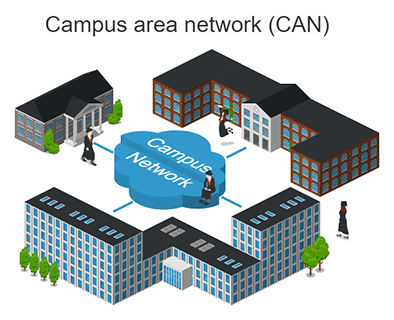
\includegraphics[scale=0.60]{Chapter1/campusNetwork}
\caption{A Campus Network}
\label{figure1}
\end{center}
\end{figure}
\noindent For this reason, computer networks play a vital role in the education
area by providing efficient communications for the university environment.
However, the design of computer networks differs from one university to another.
This is as a result of many factors which determine the differences. Such factors include;
adaptability, integration, resilience, security, and cost. Installing networks in a university
relies on the university�s budget, which differs by institution and from country to country.\\

For instance, there are many countries whose universities do not have the financial
capability for designing the �perfect� or ideal network. Yet these universities from these
third world countries still need to have good quality and more secure network equipment
with less cost. This is because these schools aspire to deliver capability in line with the
leading prestigious universities despite low budgets. 

\section{Motivation}
The word �digital� is very significant in today�s world, with an increase in the development of technology the entire world is moving towards the digital era. The educational institution plays an important role in this digitalization, hence the campus should adapt to digital means of networking as well and become a �digital campus�.\\

Campus networking becomes an important part of campus life and provides the main way for teachers and students to access educational resources, which gives an important platform to exchange information. As laptops and intelligent terminals are widely used, demand for access to information anytime and anywhere has become more and more urgent. Campus network provides an efficient way to explore the internet with a mobile terminal for teachers and students. This is an important mark of the modern campus. With the development of network and communication technology, cable networks on a university campus bring much convenience for teaching and research work.

%Motivated by the emergence of technological advancements and challenges in ...


%
%

%
%\section{UN Stainability Goals}

 %Goal 8 is shown which is Promote sustained, inclusive and sustainable economic growth, full and productive employment and decent work for all. As we will also discuss the economical long time benefits in next chapters. Our project will help industry in economic growth as well as it is providing a help to the meter readers.



%The conceptual frame work for the proposed method is comprises of three basic building blocks and detailed model is shown in Fig. \ref{fw}.
%\begin{enumerate}
%\item Network Formation Block.
%\item Neighbourhood Based Network Matrix Formation Block.
%\item Consensus Formation Block.
%\end{enumerate}
%
%In the network formation block, ...
%
%\FloatBarrier
%\begin{figure}[H]
%\begin{center}
%\hspace{15mm}
%\includegraphics[scale=0.35]{Chapter1/robocanesinternalstates}
%
%\protect\caption{Pseudo-code of Proposed Scheme for Cooperative Control of Networked Multi-Agent Systems.}
%\label{scode}
%\end{center}
%\end{figure}
%
%
\section{Report Break Down}
%
%This thesis deals with convergence analysis .... The main contributions of this work are summarized as follows:
%
%\begin{enumerate}
%\item  Initially a design ....
%
%\item An extended ....
%
%
%\item Modeled a ....
%
%\end{enumerate}
%
%The main contribution of this work is to propose a new way ....
%
%
%
%
%\section{Thesis Outline}
%
%
The major focus of this report is on the findings of the proposed project i.e. University Network using Cisco Packet Tracer.

This Report is organized as follows:
\vspace{5mm}

In chapter 2, literature review is provided in detail about the work which is already been done on Network using Cisco Packet Tracer and will give a brief details about the articles, papers and literature review.
\vspace{5mm}


In Chapter 3, Proposed Methodology is presented in which you will be able to see the method we will work on the designing of a complete project source code to the diagrams.

\vspace{5mm}


In Chapter 4, Result and Simulations are being discussed, in which you will see all kind of finding related to the Campus Network using Cisco Packet Tracer.

\vspace{5mm}

In Chapter 5, we have concluded and summarized the project work and also presented few new research ideas for future studies.


%\begin{equation}
%F=\sum_{n=0}^i(x_i(0)-x_j(0))^2
%%stackrel[u]{v}{T}=\stackrel[u]{v}{L}+\stackrel[u]{v}{L}\underset{W\epsilon V\cap w\neq u}{\sum}\stackrel[v]{w}{L}
%\end{equation}

\chapter{Literature Review}
\label{chap2}
In the chapter 1 we have given the introduction of our project, objectives and a thesis break down. Our introduction chapter is giving a complete overview of this project report. This chapter is about the work which is already been done on University Network using Cisco Packet Tracer, and will give a brief details about the articles, papers and literature review.

\section{Literature Review}
This chapter is about studies and literatures that are related to the University Network using Cisco Packet Tracer that the proponents made use of different reading materials (such as thesis, articles, and other web articles) that will help extending the knowledge of the topic. These reading materials will also guide the proponent to improve and develop their proposed system more effectively.

\subsection{Network Topology}
A network topology defines how hosts are connected to a computer network. It
characterizes how the PCs and other hosts are organized, and linked to each other.
\subsubsection{Point to Point Topology}
Point to Point topologies connect two computers together with a single line
connection. The advantage of Point to Point Topology is that it gives a faster connection,
and it is also less expensive than other topologies. The strength of this topology is more
than other kinds of connection\cite{kornilovitch2009fully}.\\
\begin{figure}[H]  %h=positioning
\begin{center}
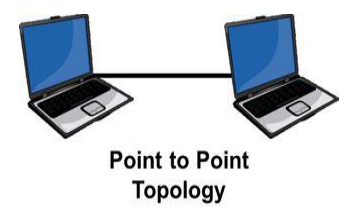
\includegraphics[scale=0.62]{Chapter1/pTopTopology}
\caption{Point to Point Topology}
\label{figure1}
\end{center}
\end{figure}

\subsubsection{Bus Topology}
Bus topology, with the inexpensive configuration, many computers are connected
by a single line of cable. Each side of the main cable must be connected to terminals.
This type of network topology is small and very easy to connect devices together to
making the network. The bus topology uses one main cable for all the connection, and
it�s usually seen in smaller networks. If the main cable is broken, there will be a network
failure such as that seen at a local office level\cite{alsarhan2016computer}.\\

\begin{figure}[H]  %h=positioning
\begin{center}
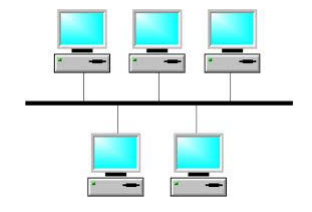
\includegraphics[scale=0.80]{Chapter1/busTopology}
\caption{Bus Topology}
\label{figure1}
\end{center}
\end{figure}

\subsubsection{Ring Topology}
Another topology is the ring topology, which uses a connecting computer in a circle
shape. The source computer sends information to the cable ring, and this information
searches for its destination by accessing each computer on the ring until it gets its
destination node. According to the article ``A review of Network Topology'' by Jiang,
�Adjacent pairs of workstations are directly connected. Other pairs of workstations are
indirectly connected, the data passing through one or more intermediate nodes \cite{jiang2015review}.''
\begin{figure}[H]  %h=positioning
\begin{center}
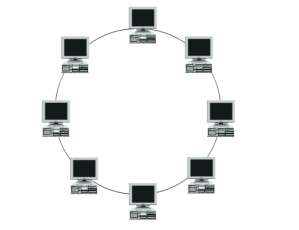
\includegraphics[scale=0.90]{Chapter1/ringTopology}
\caption{Ring Topology}
\label{figure1}
\end{center}
\end{figure}

\subsubsection{Mesh Topology}
The mesh topology requires each computer to be connected directly to multiple
computers, with more than one line connecting all computers to each other. One good
thing about this topology is that if one line fails or cut, it will use the other paths to send
information to the destination. This reduces the probability of a total network failure. 
Mesh topology is faster compared to other kinds of topology, but it is very expensive.
According to the Clarke ``A disadvantage of a mesh topology is the cost of the additional
cabling and network interfaces to create the multiple pathways between each system \cite{clarke2009comptia}.``\\ 
\begin{figure}[H]  %h=positioning
\begin{center}
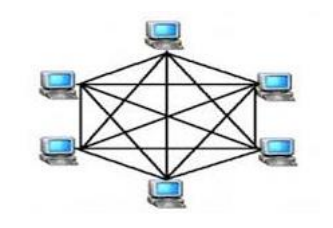
\includegraphics[scale=0.90]{Chapter1/meshTopology}
\caption{Mesh Topology}
\label{figure1}
\end{center}
\end{figure}

\subsubsection{Star Topology}
The star topology is generally used for all networks whereby each device or
computer is connected to a center hub by a direct line. The center hub can be a switch,
router, or server. Each computer connects directly to the center device such as the hub,
router, and server. ``A star topology is designed with each node connected directly to a
central network hub, switch, or concentrator \cite{jiang2015review}.'' It is easy to add
and remove a computer from the network without affecting the network. Pandya, Kartik
mentioned in their article, ``It is easy to replace, install or remove hosts or other devices,
the problem can be easily detected-It is easier to modify or add a new computer without
disturbing the rest of the network by simply running a new line from the computer to the
central location and plugging it to the hub \cite{alsarhan2016computer}.''\\

\begin{figure}[H]  %h=positioning
\begin{center}
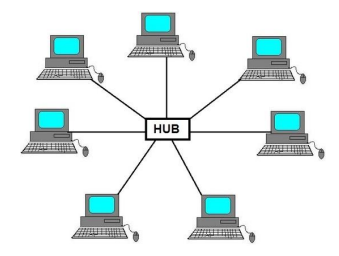
\includegraphics[scale=0.80]{Chapter1/starTopology}
\caption{Star Topology}
\label{figure1}
\end{center}
\end{figure}


%\begin{table}[H]
%%\large
%\centering
%\caption{Consolidated Comparison of all the Systems}
%\label{tab2}
%%begin{adjustwidth}{-2.25in}{Oin}
%
%\begin{tabular}{|c|c|c|c|c|c|}
%\hline  %make a line
%Technology Used&Cost&Feasibility&Reliability&Communication Protocol\\
%\hline %make a line
%GSM&Low&Most Feasible&High&Stable\\
%\hline
%ZigBee&Medium&Small Scale&Low&Least Stable\\
%\hline
%SCADA&High&Not Feasible&High&Stable\\
%\hline
%PLC&Low&Least Feasible&Low&Very Stable\\
%\hline
%WiMAX&Medium&Small Scale&Medium&Stable\\
%\hline
%Mixed&Varies&Feasible&Varies&Varies\\
%\hline
%\end{tabular}
%\end{table}
%
%\small
%\begin{table}[H]
%\caption{Literature Review}
%\label{tab3}
%\centering
%\begin{tabularx}{1\linewidth}{X X X X}
%\toprule
% Paper Reference & Approach & Technology & Accuracy ($\%$) \\
%\toprule
%\cite{khan2020cost}&Cost Benefit Based Analytical Study of AMR and Blind Meter Reading (BMR) used by PESCO(WAPDA)& AMR and BMR &The Blind Meter Reading has internal financial return of about 84 percent while in case of AMR it is 15 percent.\\
%%\toprule
%\hline  %make a line
%\cite{zhao2005research} & Remote Meter Automatic Reading
%Based on Computer Vision & Computer vision techniques & $78\%$\\
%\hline %make a line
%\cite{li2019light} & Light-Weight Spliced Convolution Network-Based
%Automatic Water Meter Reading in Smart City & Network-Based
%Automatic Water Meter Reading & $85.66\%$ \\
%%\toprule
%\hline  %make a line
%\cite{dong2010design} & Wireless AMR System Based on SOPC & SOPC & $59.6\%$ \\
%\hline  %make a line
%\cite{ando2002automatic} & AMR system adopting automatic routing technology & routing technology & $68\%$ \\
%\hline  %make a line
%\cite{wiratama2018gas} & Gas
%billing system based on AMR on diaphragm gas meter with email
%notification & GSM or
%GPRS networks & $79\%$\\
%\hline  %make a line
%\cite{ashna2013gsm} & GSM based automatic AMR system with instant billing & GSM & $88\%$\\
%\hline  %make a line
%\cite{shuo2019digital} & Digital recognition of electric meter with deep learning & Deep Learning Methods & $78\%$\\
%\hline  %make a line
%\end{tabularx}
%\end{table}
%\small
%\begin{table}[H]
%\caption{-- continued from previous Literature Review table \ref{tab3}}
%\label{tab4}
%\centering
%\begin{tabularx}{1\linewidth}{X X X X}
%\toprule
% Paper Reference & Approach & Technology & Accuracy ($\%$) \\
%\toprule
%
%\cite{kulkarni2012gsm} &GSM based AMR system using ARM controller & ARM Controller & $81\%$\\
%\hline  %make a line
%\cite{Ali2012} & Implementation of (AMR) using radio frequency (RF) module & Radio Frequency & $58\%$\\
%\hline  %make a line
%\cite{palaniappan2015automated} & Comparison between different technologies being used in ARM  & GSM, Zigbee, SCADA System, Power Line Communication, WiMAX Technology,  & GSM = $88\%$, Zigbee = $67\%$,SCADA = $63\%$,Power Line = $71\%$,WiMAX = $62\%$,  \\
%\hline %make a line
%\cite{quan2010design} & Design of remote automatic meter reading system based on ZigBee and GPRS & ZigBee and GPRS techniques & $67\%$\\
%\hline  %make a line
%\cite{arun2012design} & Design and implementation of AMR system using GSM, ZIGBEE through GPRS & using GSM, ZIGBEE through GPRS & $89\%$\\
%\hline  %make a line
%\cite{rouf2012neighborhood} & Security and privacy analysis of automatic meter reading systems & Analysises of AMR & -\\
%\hline  %make a line
%\cite{malhotra2013automatic} & AMR and theft control system by using GSM & GSM & $84\%$\\
%\hline  %make a line
%\cite{tan2007automatic} & Automatic power meter reading system using GSM network & GSM network  & $78\%$\\
%\hline  %make a line
%\cite{Jamil2008} & Design and implementation of a wireless AMR system & GSM Network & $86\%$\\
%\hline  %make a line
%\cite{yuan2011remote} & Remote wireless AMR system based on GPRS & GPRS & $88\%$\\
%\hline  %make a line
%\cite{borle2013automatic} & AMR for electricity using power line communication & power line communication & $65\%$\\
%\hline  %make a line
%\end{tabularx}
%\end{table}
%\small
%\begin{table}[H]
%\caption{-- continued from previous Literature Review table \ref{tab4}}
%\label{tab5}
%\centering
%\begin{tabularx}{1\linewidth}{X X X X}
%\toprule
% Paper Reference & Approach & Technology & Accuracy ($\%$) \\
%\toprule
%\cite{mlakic2017designing} & Designing AMR system using open source hardware and software &open source hardware and software & $59\%$\\
%\hline  %make a line
%\cite{khalifa2010survey} & A survey of communication protocols for auto-
%matic meter reading applications, & Communication Protocols & - \\
%\hline
%\bottomrule
%\end{tabularx}
%\end{table}

%\section{Concluding Remarks}
%In this chapter, we have given a overall review about the literature related to Speech Processing Using MATLAB. MATLAB is a programming and numeric computing platform used by millions of engineers and scientists to analyze data, develop algorithms, and create models.\\\\
%In the chapter 3 we will proposed methodology which we will use for our project with block diagrams, flowcharts, Mathematical Modeling, escudo code and component selection related to the hardware and software.


\chapter{Proposed Methodology}
\label{chap3}

In the previous chapter, we have discussed the theories that support this
research related to the University Network using Cisco Packet Tracer. In this chapter we will proposed our methodology for this project.\\\\
Basically we are following the given below question step by step.\\
COMSATS University is a large university which has 4 main buildings situated apart. The university's students and staff are distributed in 4 departments: these includes the Department of Electrical and Computer Engineering, Department of Mathematics, Department of Computer Sciences, \& Admission Office.\\\\
Each member of staff has a PC and students have access to PCs in the labs.\\\\
\noindent {\Large \textbf{Requirements}} \\
\begin{itemize}
\item Create a network topology with the main components to support the following:
    \begin{enumerate}
    \item {\small \textbf{Building A}}: Department of Electrical and Computer Engineering is distributed in the building offices for the faculty, and labs. It is expected that they will share networking equipment ({\small \textbf{Hint: use of VLANs is expected here}})
    \item {\small \textbf{Building B}}: Department of Mathematics including offices, lecture halls/lecture rooms.
%
    \item {\small \textbf{Building C}}: Admission office distributed in different offices.
    \item There is also an email server hosted externally on the cloud.
    \item {\small \textbf{Building D}}: Department of Computer Sciences (CS) this can acts as a smaller campus as well as. It includes different offices and labs.
%
\end{enumerate}
\item You will be expected to configure the core devices and few end devices to provide end-to-end connectivity and access to the internal servers and the external server.
    \begin{enumerate}
    \item Each department/faculty is expected to be on its own separate IP network
    \item The switches should be configured with appropriate VLANs and security settings
    \item RIPv2 will be used to provide routing for the routers in the internal network and static routing for the external server.
    \item The devices in building A will be expected to acquire dynamic IP addresses from a router-based DHCP server
%
\end{enumerate}
\end{itemize}

\section{Block Diagram}
Let us look at the detail block diagram in Figure \ref{blockDiagram}, which illustrates the main components involved
in University Network using Cisco Packet Tracer.\\
In this diagram, we have used:
\begin{enumerate}
    \item 2911 Router, for the main campus network
    \item 3650-24PS Multi Layer Switch, for different departments in the buildings 
    \item 2960-24TT Switches, for each department 
    \item A cloud router,
    \item Servers, email server hosted externally on cloud, and a web server for IT department
    \item Host Devices, a PC and a printer 
    \item Wire, Serial DCE (HWIC-2T) for routers connections, Copper cross over for switches connections, and Copper straight through for the host devices connections.
%
\end{enumerate}
 
\begin{figure}[H]  %h=positioning
\begin{center}
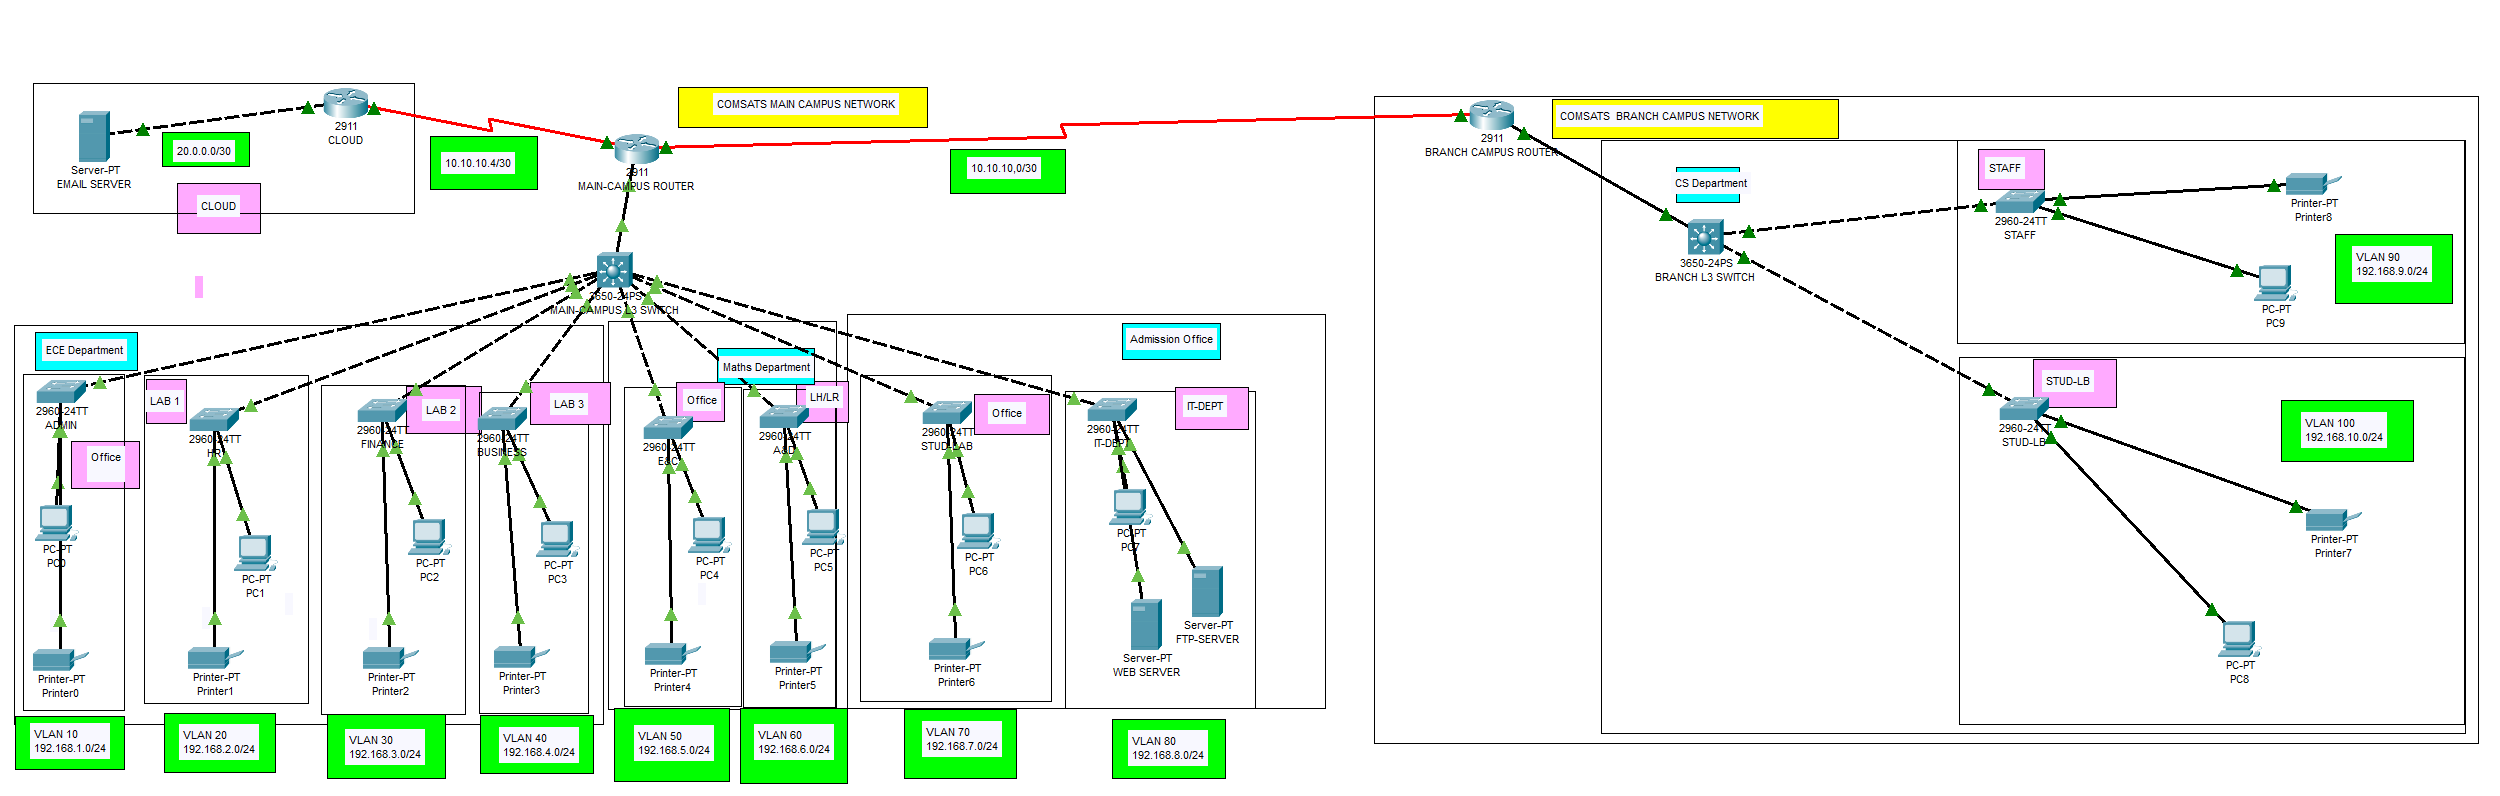
\includegraphics[scale=0.24]{Chapter3/blockDiagram}
\caption{Block Diagram of University Network }
\label{blockDiagram}
\end{center}
\end{figure}

\section{Flow Chart}
Figure \ref{flowChart} shows the flow chart of the University Network. Basically the main objective of the project is the communication between different departments. To do so, we send message from one of the department's pc to any other department's pc or printer.\\\\
We will configure the network first, and than will check out if the IP of the next computer and our computer is working well. It will transfer our message packet to the destination host.
\begin{figure}[H]  %h=positioning
\begin{center}
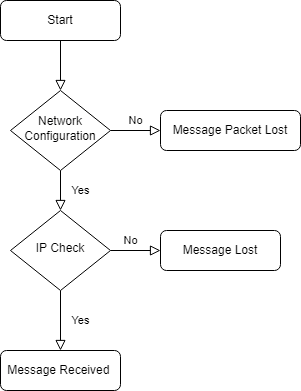
\includegraphics[scale=0.70]{Chapter3/flowChart}
\caption{Flow Chart of University Network }
\label{flowChart}
\end{center}
\end{figure}

\section{System Model}
A large campus with groups of buildings can also use WAN technology to connect the buildings as shown in the Fig. \ref{systemModel}. Although the wiring and protocols of a campus might be based on WAN technology, they do not share the WAN constraint of the high cost of bandwidth. After the wire is installed, bandwidth is inexpensive because the company owns the wires and there is no recurring cost to a service provider. However, upgrading the physical wiring can be expensive.
\begin{figure}[H]  %h=positioning
\begin{center}
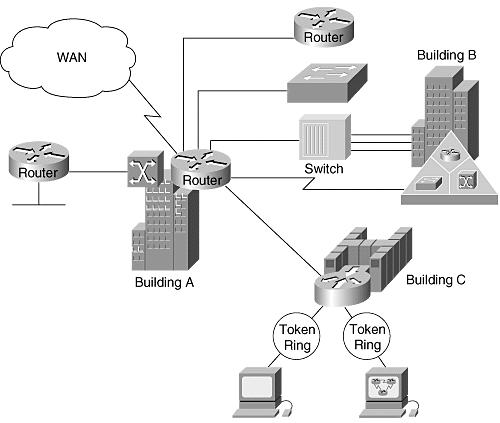
\includegraphics[scale=0.67]{Chapter3/systemModel}
\caption{System Model of University Network}
\label{systemModel}
\end{center}
\end{figure}
\section{Software Selection}
We will simulate our campus network using Cisco Packet Tracer Version: 7.3.0.0838. Cisco Packet Tracer is a powerful network simulator for CCNATM and CCNPTM certification exam training allowing students to create networks with an almost unlimited number of devices and to experience troubleshooting without having to buy real CiscoTM routers or switches.\\

\noindent Cisco Packet Tracer features an array of simulated routing \& switching protocols with STP, HSRP, RIP, OSPF, EIGRP, and BGP to the extent required by the current Cisco CCNA curriculum as well as application layer protocols (HTTP, DNS, �) to simulate network trafic .\\

\noindent It also includes Cisco IOS 15 with licence features, wireless capabilities with WLC and lightweight access point, security devices with ASA 5505 and 5506-X firewalls, and SDN controller.
\begin{figure}[H]  %h=positioning
\begin{center}
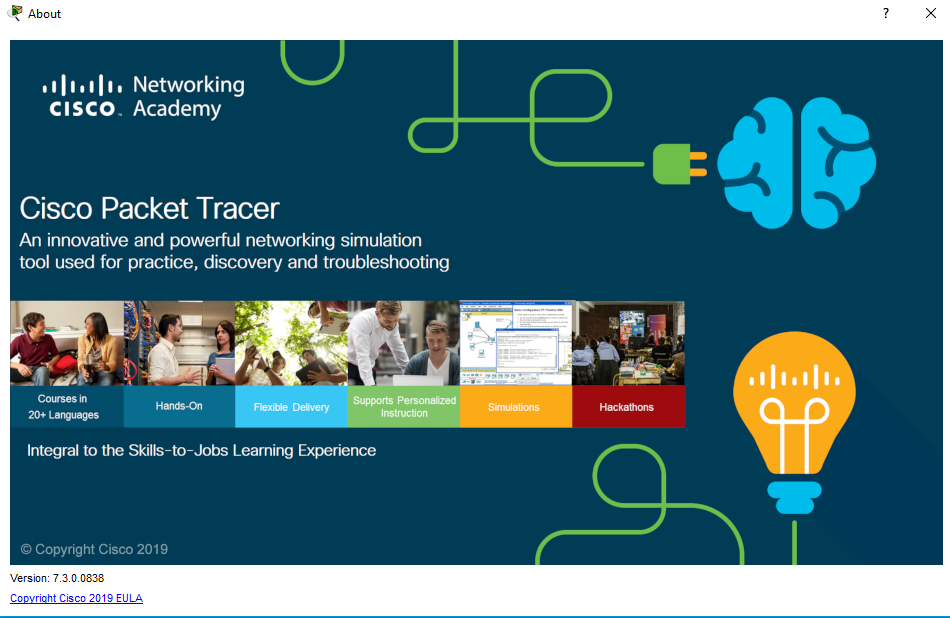
\includegraphics[scale=0.60]{Chapter3/software}
\caption{Cisco Packet Tracer}
\label{software}
\end{center}
\end{figure}

{ \small \bfseries Note: You can simulate this network on any latest version as well as.}



\chapter{Simulation and Results}
\label{chap4}
In the previous chapter, we have discussed about our methodology for this project while giving details about block diagram, system model, flow chart, software selection of this project. In this chapter, we will provide the viewable logical topology, and results of the project.
\section{Simulation Results}
As discussed in the previous chapter in the section of software selection, we have used Cisco Packet Tracer to simulate our project.
\subsection{Logical Topology}
In the Fig. \ref{mainBranchCampus} a main branch topology is shown which contain three departments, Electrical and Computer Engineering Department, Mathematics Department, Admission Department, and a Cloud Server.
\begin{figure}[H]  %h=positioning
\begin{center}
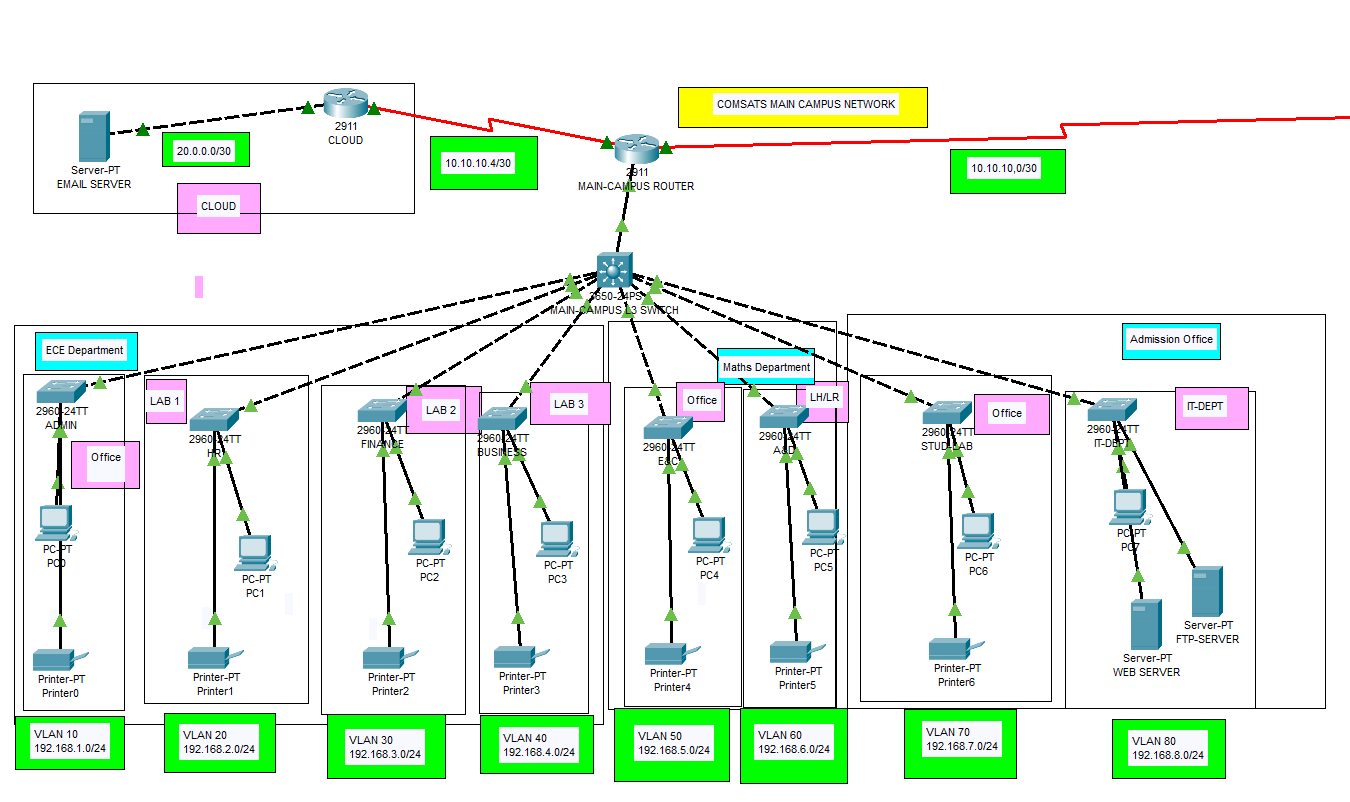
\includegraphics[scale=0.43]{Chapter4/mainBranchCampus}
\caption{Main Branch Topology}
\label{mainBranchCampus}
\end{center}
\end{figure}
Whereas in Fig. \ref{branchCSDepartment}, department of Computer Science is shown which contains different offices and lab. The reason we called this COMSATS Branch Campus is because it is quite apart from the other department in this case we can consider this as a Branch Campus. We can include this in the main branch too but the reason of treating this as a campus is to learn how to connect campus network with the main network.
\begin{figure}[H]  %h=positioning
\begin{center}
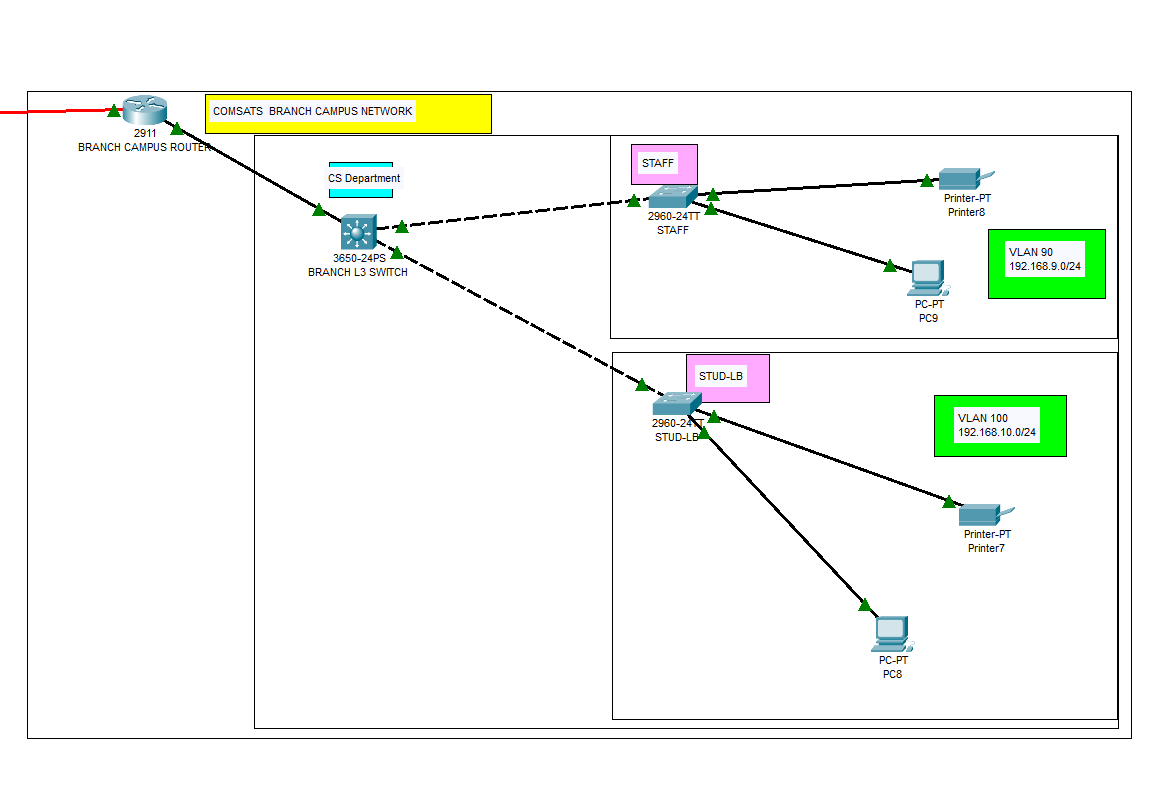
\includegraphics[scale=0.50]{Chapter4/branchCSDepartment}
\caption{Branch Topology of CS Department}
\label{branchCSDepartment}
\end{center}
\end{figure}
\subsection{Statistical Analysis}
\label{analysis}
Fig. \ref{resultSimulation} shows the results of the simulation. In which, we have forwarded a message from source host i.e., PC0 to the destination host i.e., PC4.\\
\begin{figure}[H]  %h=positioning
\begin{center}
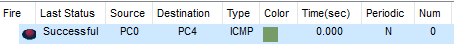
\includegraphics[scale=1.3]{Chapter4/resultSimulation}
\caption{Simulation Results}
\label{resultSimulation}
\end{center}
\end{figure}
Fig. \ref{simulationPanel} it's showing a complete path which it follows to reach to the destination host and than acknowledge back to the source host with the time it take while using Internet Control Message Protocol (ICMP) which is a network layer protocol used by network devices to communicate.
\begin{figure}[H]  %h=positioning
\begin{center}
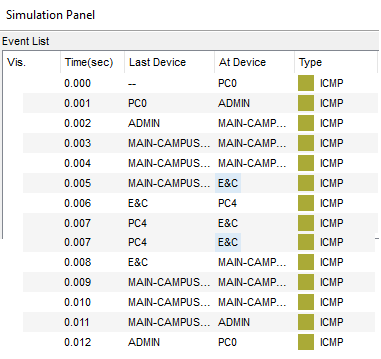
\includegraphics[scale=1.0]{Chapter4/simulationPanel}
\caption{Simulation Panel Results}
\label{simulationPanel}
\end{center}
\end{figure}
\subsection{Using Command Prompt}
\noindent The ping command is a very common method for troubleshooting the accessibility of devices. It uses a series of Internet Control Message Protocol (ICMP) Echo messages to determine:\\
\begin{itemize}
\item Whether a remote host is active or inactive.

\item The round-trip delay in communicating with the host.

\item Packet loss.
\end{itemize}

\noindent The ping command first sends an echo request packet to an address, then waits for a reply. The ping is successful only if:
\begin{itemize}
\item the echo request gets to the destination, and

\item the destination is able to get an echo reply back to the source within a predetermined time called a timeout. The default value of this timeout is two seconds on Cisco routers.
\end{itemize}
\noindent Fig. \ref{commandPrompt} shows a different way to check if our network connectivity is reliable. We have used command prompt of PC2 and have ping two hosts: one from the branch/CS Department host i.e, PC8 with IP address 192.168.10.2/24 and second from Admission Department host's i.e., PC6 with IP address 192.168.7.2/24.
\begin{figure}[H]  %h=positioning
\begin{center}
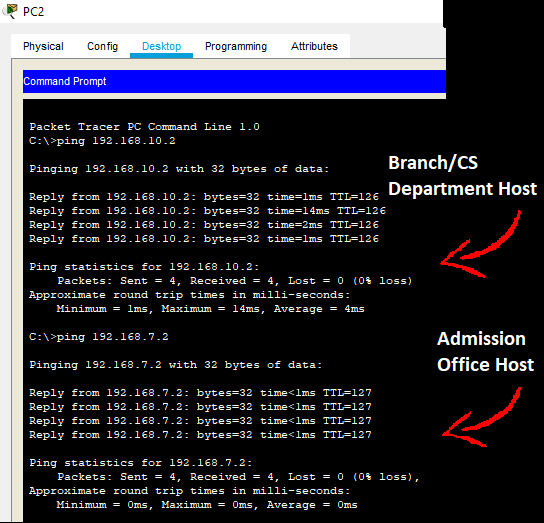
\includegraphics[scale=1.0]{Chapter4/commandPrompt}
\caption{Command Prompt Results}
\label{commandPrompt}
\end{center}
\end{figure}




\chapter{Conclusion and Future Work}
\label{chap5}
In the previous chapter, we have shown all the simulation and results of our proposed project. From introduction, Literature Review, Proposed Methodology, Result and Simulations. In this chapter, we will conclude our project and will
\section{Conclusion}
This work describes the COMSATS University Islamabad, Attock Campus Network. We have:
\begin{enumerate}
\item Successfully simulated our topology using Cisco Packet Tracer.
%
\item Learned basic knowledge of how department communicate with each other in any organization.
%
\item Discussed a real life university scenario.
%
\end{enumerate}
In this project, we have done following tasks:
\begin{enumerate}
\item Planned, designed, and prototyped the network topology for our university i.e., COMSATS University Islambad, Attock Campus.
%
\item Configured the network in Cisco Packet Tracer with appropriate settings to acheive the connectivity and functionalities.
%
\end{enumerate}

\section{Future Work}

For future work, we recommend the Following things:

\begin{enumerate}
\item Practical implementation of the network.
%
\item Work on the security of the network.
%
\item Can simulate the network on any other simulation software.
%
\item Can work on the accuracy and time of the received signal.
\end{enumerate}


%\include{Chapter6/Chapter6}
%\include{Chapter8/Chapter8}
%\include{Chapter7/Chapter7}

\bibliographystyle{ieeetr}
\bibliography{Ref}
\end{document}
